\section{Examples in videos for different dog vocal patterns}
For each word audio file, you can check the anonymous website \footnote{\url{https://anonymous.4open.science/r/emnlp2023-937942/audios_in_paper/}}.
\begin{figure}[ht]
        \centering
        \includegraphics[width=0.6\columnwidth]{images/whimper_attention.png}
        \caption{Dog whimpers to seek attention from host for food. \href{https://anonymous.4open.science/r/emnlp2023-937942/audios_in_paper/whimper-food.wav}{[Listen]}}
        \label{fig:whimper_attention}
\end{figure}

\begin{figure}[ht]
        \centering
        \includegraphics[width=0.6\columnwidth]{images/bark_cage.png}
        \caption{Dog barks when located in the cage to show anger.\href{https://anonymous.4open.science/r/emnlp2023-937942/audios_in_paper/bark-cage.wav}{[Listen]}}
        \label{fig:bark_cage}
\end{figure}

\begin{figure}[ht]
        \centering
        \includegraphics[width=0.6\columnwidth]{images/bow-wow_snowfield.png}
        \caption{Dog bow-wows in the snowfield.\href{https://anonymous.4open.science/r/emnlp2023-937942/audios_in_paper/bowwow-snowfield.wav}{[Listen]}}
        \label{fig:bow-wow_snowfield}
\end{figure}

\begin{figure}[ht]
	\centering
	\includegraphics[width=0.6\columnwidth]{images/bowwow_walking.png}
	\caption{Dog bow-wows because of movements.\href{https://anonymous.4open.science/r/emnlp2023-937942/audios_in_paper/bowwow-walking.wav}{[Listen]}}
	\label{fig:bow-wow_walking}
\end{figure}

\begin{figure}[ht]
	\centering
	\includegraphics[width=0.6\columnwidth]{images/howl_food.png}
	\caption{Dog howls because of food.\href{https://anonymous.4open.science/r/emnlp2023-937942/audios_in_paper/howl-food.wav}{[Listen]}}
	\label{fig:howl_food}
\end{figure}

\begin{figure}[ht]
	\centering
	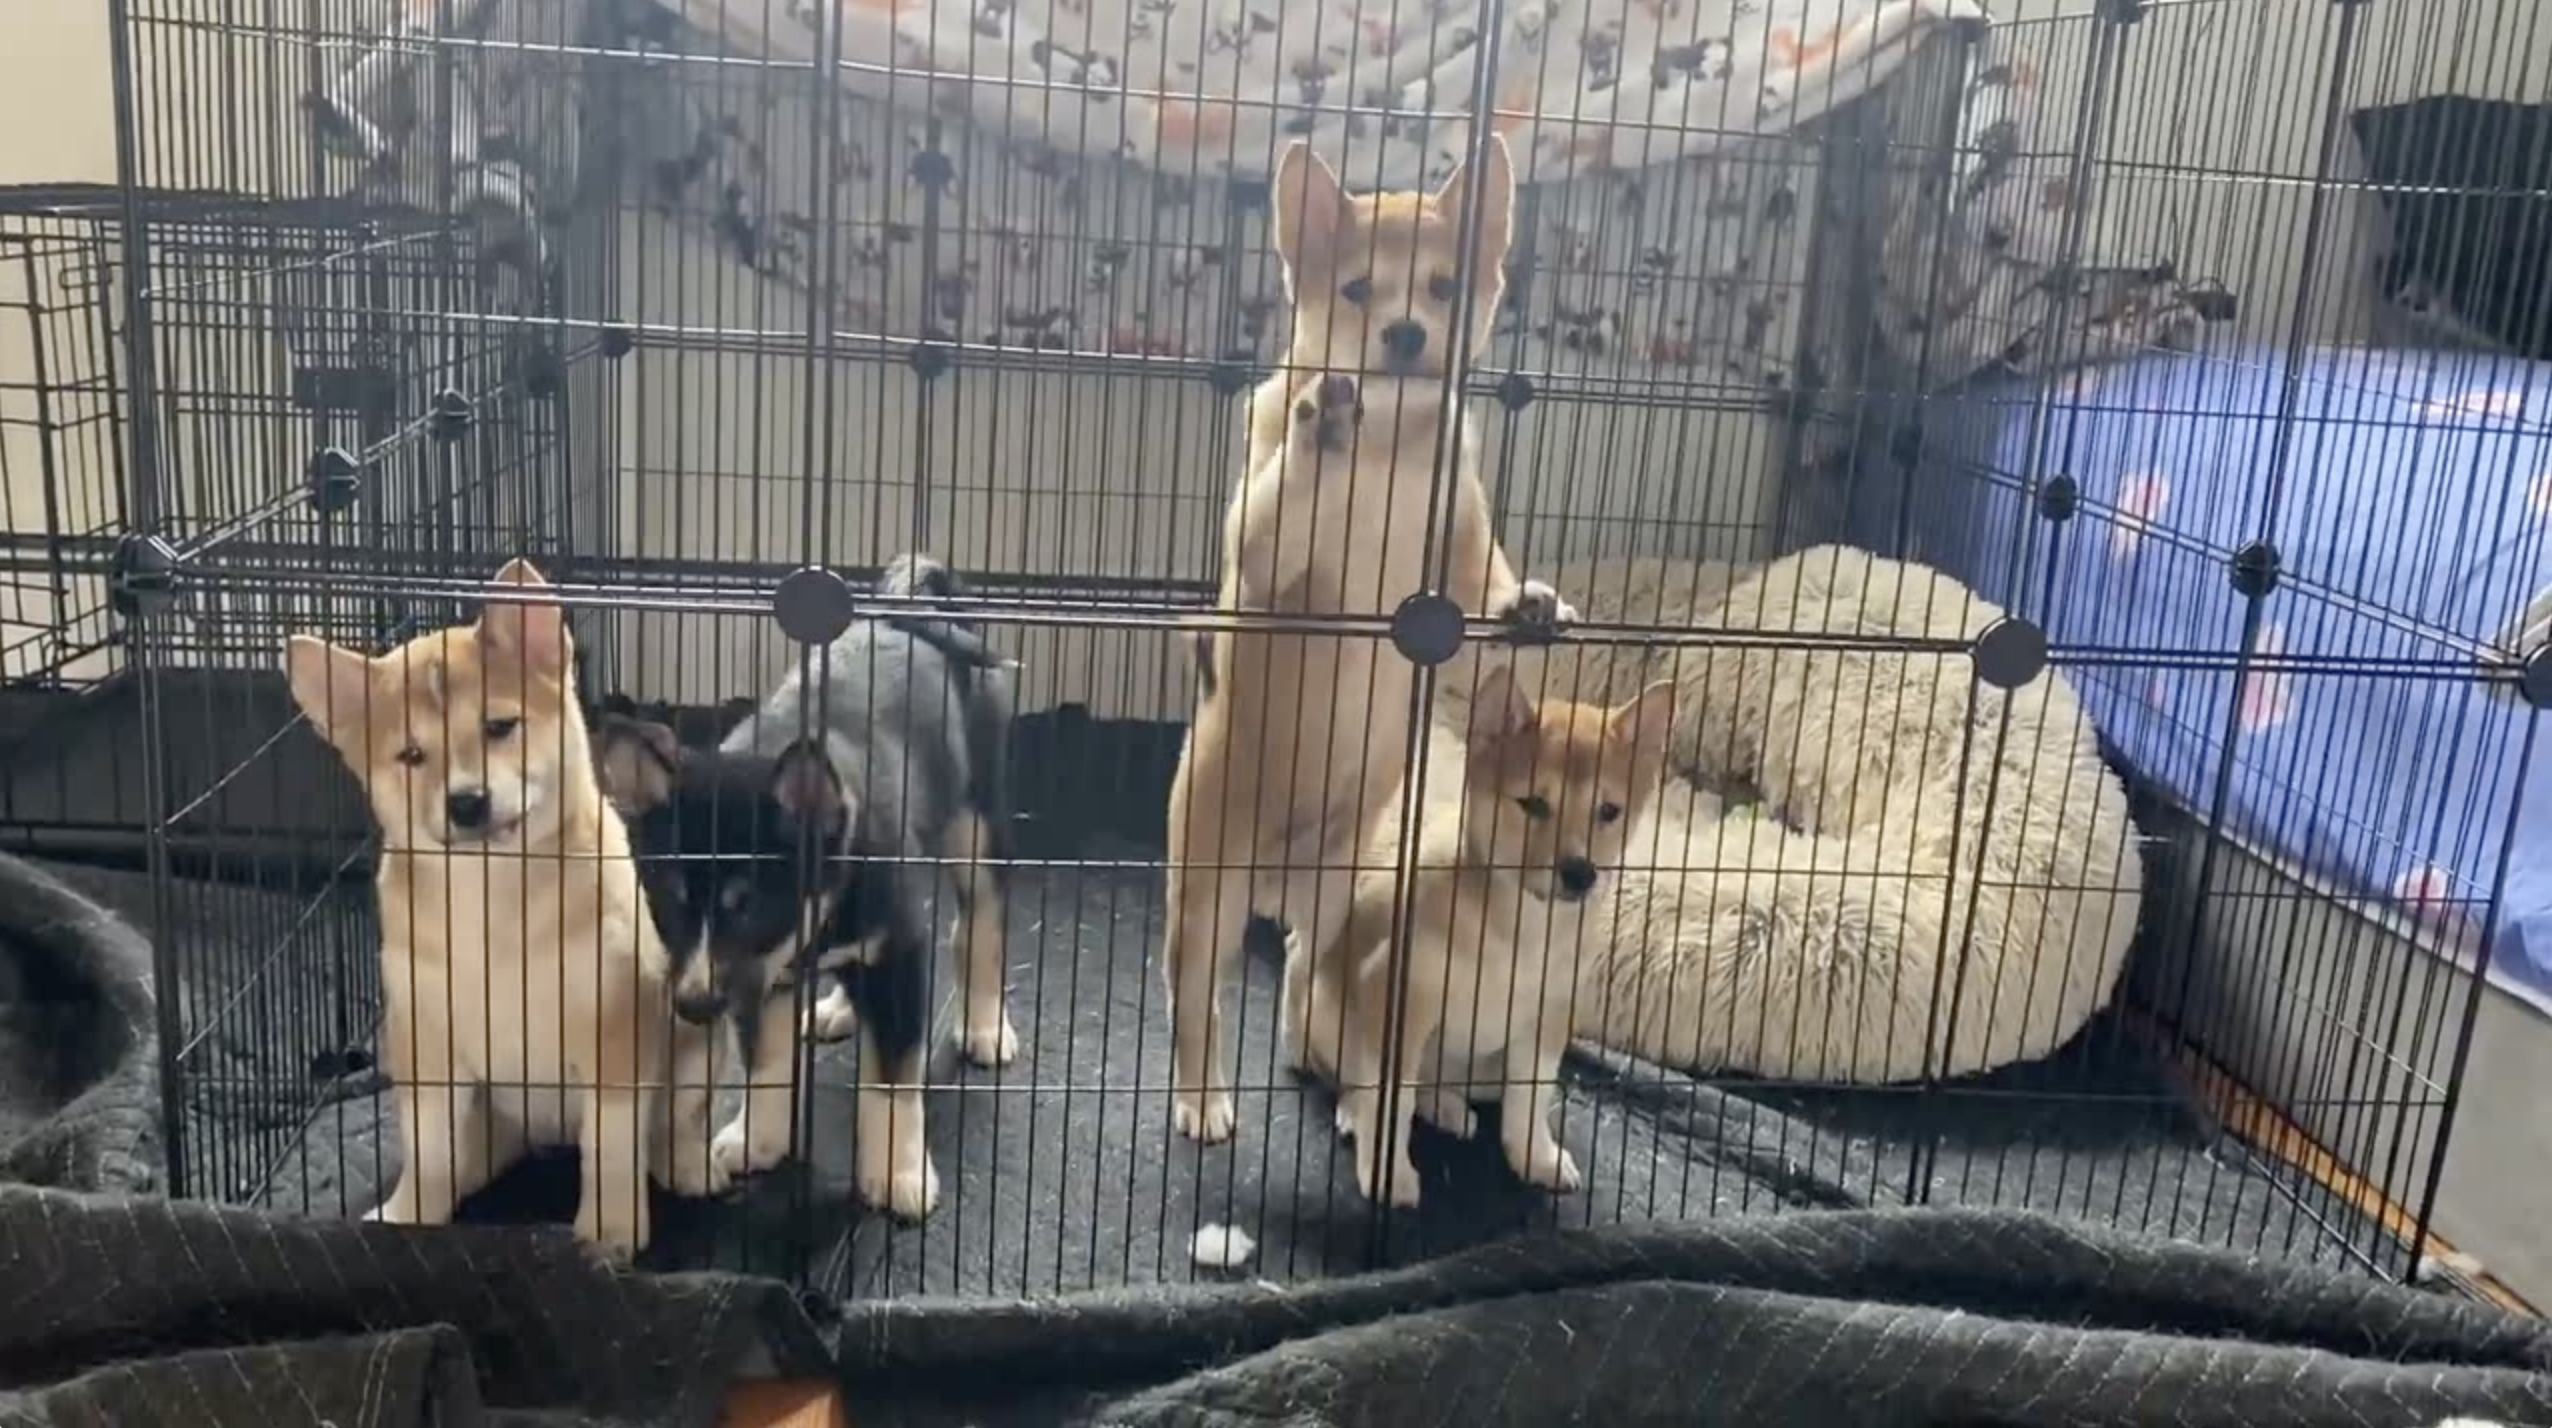
\includegraphics[width=0.6\columnwidth]{images/yip_cage.png}
	\caption{Dog yips when staying in the cage.\href{https://anonymous.4open.science/r/emnlp2023-937942/audios_in_paper/yip-cage-layingdown.wav}{[Listen]}}
	\label{fig:yip_cage}
\end{figure}

\begin{figure}[ht]
	\centering
	\includegraphics[width=0.6\columnwidth]{images/growl_play.png}
	\caption{Dog growls when playing with human.\href{https://anonymous.4open.science/r/emnlp2023-937942/audios_in_paper/growl-play.wav}{[Listen]}}
	\label{fig:growl_play}
\end{figure}

\begin{figure}[ht]
	\centering
	\includegraphics[width=0.6\columnwidth]{images/whimper_bow-wow.png}
	\caption{Dog whimpers then bow-wows for asking food.\href{https://anonymous.4open.science/r/emnlp2023-937942/audios_in_paper/whimper-bowwow-food_1.wav}{[Listen 1]} \href{https://anonymous.4open.science/r/emnlp2023-937942/audios_in_paper/whimper-bowwow-food_2.wav}{[Listen 2]}}
	\label{fig:Whimper_Bow-wow_food}
\end{figure}

\section{Figure for bi-gram probability}
\label{sec:bigram}
%We make two observationss here. First, ``Bark'' and ``bow-wow'' show a 
%similar distribution of relative probability and this shows that these two 
%expressions may share similar semantics. ``Whimper'' and ``Yip'' may also 
%convey the same semtantics for similar distribution. Second, for ``growl'' 
%and ``howl'', they are always followed by exactly the same word, 
%implying that these words each contain a special meaning. 

\begin{figure*}[th]
    \centering
    \begin{subfigure}[b]{0.3\textwidth}
	\centering
    	\includegraphics[width=\textwidth]{images/Bark.png}
	\caption{Bigram: Bark;*}
    \end{subfigure}
    \begin{subfigure}[b]{0.3\textwidth}
	\centering
	\includegraphics[width=\textwidth]{images/Bow-wow.png}
	\caption{Bigram: Bow-wow;*}
    \end{subfigure}
    \begin{subfigure}[b]{0.3\textwidth}
	\centering
    	\includegraphics[width=\textwidth]{images/Growl.png}
	\caption{Bigram: Growl;*}
    \end{subfigure}
    \begin{subfigure}[b]{0.3\textwidth}
	\centering
    	\includegraphics[width=\textwidth]{images/Howl.png}
	\caption{Bigram: Howl;*}
    \end{subfigure}
    \begin{subfigure}[b]{0.3\textwidth}
	\centering
    	\includegraphics[width=\textwidth]{images/Whimper.png}
	\caption{Bigram: Whimper;*}
    \end{subfigure}
    \begin{subfigure}[b]{0.3\textwidth}
	\centering
    	\includegraphics[width=\textwidth]{images/Yip.png}
	\caption{Bigram: Yip;*}
    \end{subfigure}
    \caption{Bi-gram sequence probabilities.}
    \label{tab:bigramword}
\end{figure*}

